\par This chapter discusses the methodology used to measure the effectiveness of \ac{ARG} at correctly classifying invalid and valid traffic, the maximum supportable hop rate at various network latencies, and the overall stability of the system under test. Section \ref{sec:problem_def} discusses the problem this research seeks to answer. Section \ref{sec:boundaries} defines the \ac{SUT} and Section \ref{sec:services} goes into detail on the possible outcomes of the \ac{CUT}. Section \ref{sec:workload} covers the workload presented to the \ac{SUT}, Section \ref{sec:metrics} covers the metrics collected, and Section \ref{sec:parameters} covers the configurable parameters of the \ac{SUT}. Section \ref{sec:factors} brings the previous sections together, giving a comprehesive list of the factors varied for each test. Section \ref{sec:exp_design} details the actual tests and the purpose of each.

\section{Problem Definition}
\label{sec:problem_def}
\subsection{Goals and Hypothesis}
\label{sec:goals}
\par This research seeks to test whether network address space randomization is a suitable for deployment on a military network. As such, chapter 3 presents the details of custom solution that fuses much of the previous research with the needs of the military. Tests against this system seek to answer four basic questions.  First, does \ac{ARG} classify traffic correctly? What percentage of false positives (valid packets blocked) and false negatives (invalid traffic allowed through) does it introduce? Second, what is the max packet rate \ac{ARG} can handle? Third, what is the max hop rate---the frequency with which \ac{ARG} changes \acp{IP}---that is supportable? How does latency affect this? Fourth and finally, is \ac{ARG} stable when presented with corrupt, malformed, or replayed packets?

%\par The software developed and tested here attempts to interfere minimally with the network, a critical requirement for the real-world deployment of such technology. Systems \ac{ARG} touches---both inside and outside the ``protected'' networks---do not need any modifications to continue to function. The research done here provides data on whether this is true as a side effect, potentially valuable information for an organization considering employing a \ac{DYNAT} solution. However, validation of this design goal is not a primary objective. 

%\par The working hypothesis for this research is, as speculated by Sandia, a \ac{DYNAT} system allows for quick identification of unexpected (and potentially malicious) packets entering a network. There are few identifiers within the scope of \ac{DYNAT} by which outgoing packets could be filtered. Given that, no filtering is done for outbound packets and hence no change in behavior is observed when compared to the control network. 

\par It is hypothesized that \ac{ARG} correctly classifies 99\% of traffic it encounters when operating with a hop rate appropriate for the network latency. In addition, this thesis hypothenizes that the max hop rate sustainable with reasonable loss is twice the network latency, where reasonable loss is traffic loss less than 5\%. The other two questions under test are informational in nature, but it is believed that \ac{ARG} is stable in the face of malformed traffic and it can handle at least 1Mbps of traffic. \tbd{performance wasn't really a design focus} 

\subsection{Approach}
\label{sec:approach}
\par This research is done on a test network with nodes representing the types of hosts found on a typical, corporate-style network. These include trusted hosts inside trusted networks which communicate freely, internal and external servers that must be accessible to hosts inside these trusted networks, and malicious hosts outside the networks. A configurable custom \ac{DYNAT} sits in front of the trusted networks. \tbd{diagram for last sentence}

\par Traffic generators and collectors run on this network, determining which traffic flows successfully make it to their destination. More importantly, they compare what should have been denied to what \ac{ARG} actually denied (Type I and Type II errors). After a given test, logs and traffic captures are collated to form a complete picture of the traffic on the network before determining statistics.

\FloatBarrier
\section{System Boundaries}
\label{sec:boundaries}
\par The \ac{SUT} is \ac{ARG}, the custom \ac{DYNAT} solution developed specifically for this effort. The basic components of this system, the various inputs into the system, possible outputs, and the metrics provided are illustrated in Figure \ref{fig:sut}. Many traditional network workload and system parameters are not shown here, such as packet rate, packet size, and link bandwidth. In most cases these are controlled to fit \ac{ARG}, as the performance of the system itself is not a primary focus of the research. See Section \ref{sec:workload} for more details on this decision. The only system parameter this research is concerned with is latency, as it dictates the maximum \ac{IP} hopping rate.

\tbd{fix this}
\begin{figure}
	\caption{Address Routing Gateway}
	\label{fig:sut}
	\centering
	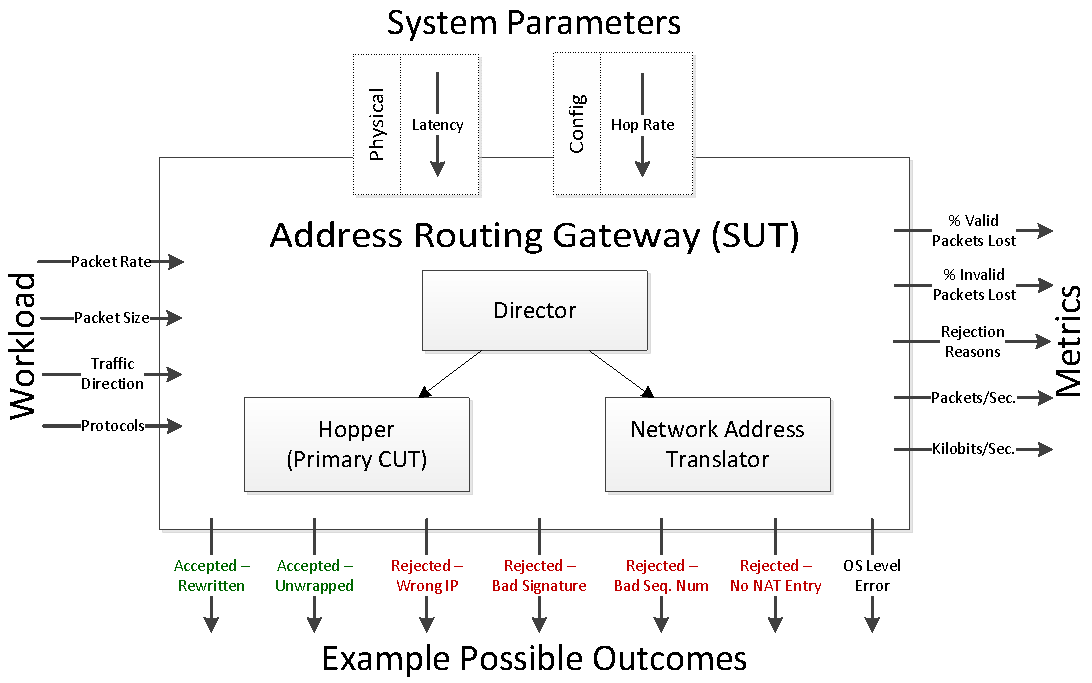
\includegraphics[width=1\textwidth]{../diagrams/sut}
\end{figure}

\FloatBarrier
\section{System Services}
\label{sec:services}
\par \ac{ARG} has three components that this thesis tests. Most important is the hopper module, which provides a rapidly-changing external IP address and details on connected ARG networks. Using this information, it transports packets between ARG-protected networks. Packets to and from external hosts---hosts that are not part of an ARG network---go through the \ac{NAT} module. The director module hands packets off to each of the other modules and collects the results back to be logged and potentially acted upon. More details on these components are in Chapter \ref{chp:implementation}.

\par The potential output of the Director is shown below, broken into separate sections based on incoming or outgoing packets. Other services do not directly offer outcomes relevant to this research.

\begin{itemize}
\item Director - Incoming
	\begin{itemize}
	\item Incorrect source \ac{IP} - Packet is coming from an \ac{ARG} network but does not have the what the local gateway believes is the current source IP for the other gateway.
	\item Incorrect destination \ac{IP} - Packet is coming from an \ac{ARG} network but does not have the current local gateway \ac{IP} as the destination.
	\item Incorrect message size - The message length does not match the message type.
	\item Incorrect sequence number - The message's sequence number was not monotonically increasing. 
	\item Unable to verify signature/\ac{HMAC} - Packet signature invalid/nonexistent (if coming from an \ac{ARG} network).
	\item Unwrapped and forwarded - Packet is from \ac{ARG} network and passed the above tests. Contents are extracted and forwarded internally.

	\item No \ac{NAT} bucket/entry - Packet is coming from a non-\ac{ARG} network but does not have a valid entry in the \ac{NAT} table.
	\item Rewritten and forwarded - Packet is from non-\ac{ARG} network and is rewritten via \ac{NAT} table before forwarding.

	\item Misc - Some operating system levels may occur, resulting in rare errors in sending or receiving packets.
	\end{itemize}

\item Director - Outgoing
	\begin{itemize}
	\item Gateway not connected - Packet was intended for an ARG network the gateway is aware of but not yet connected to.
	\item Wrapped and forwarded - Packet is destined for an \ac{ARG} network. Wrapped and placed on the external network.

	\item Rewritten and forwarded - Packet is destined for non-\ac{ARG} network. An entry is made/retrieved from the \ac{NAT} table and used to rewrite packet.

	\item Misc - Some operating system levels may occur, resulting in rare errors in sending or receiving packets.
	\end{itemize}
\end{itemize}

\section{Workload}
\label{sec:workload}
\par Workload to the system is the traffic flowing through the \ac{ARG} gateways. Standard network traffic parameters like packet rate, packet size, number of simultaneous ongoing connections, and lifetime of connections play a role. However, it is important to note that the network performance itself is not a large concern of this research. Packet rate, for example, does provide useful information about the performance of \ac{ARG} itself, but the numbers apply \textit{only} to this specific implementation. \ac{ARG}'s develop does not focus on performance in this first iteration, so there are many possible areas for improvement. Previous research has shown that similar solutions have minimal impact on performance \cite{NAH}. 

\par The only physical network parameter that has a major impact on \ac{ARG} is latency. To ensure that two \ac{ARG} gateways are able to communicate reliably, their hop rate must be less than two times the latency. If it is not, packets sent from one to the other will have the wrong \ac{IP} by the time they reach the destination. \tbd{details on why... diagram showing traffic flow?} \tbd{Would this be an appropriate place to discuss impact of test setup (ethernet vs internet) on latency?}

\par Two parameters are more specific to \ac{ARG}. First, the proportion of inter-\ac{ARG} verses extra-\ac{ARG} traffic varies the validation methods \ac{ARG} uses for each packet. Traffic flows that focus on inter-\ac{ARG} connections rely on current \ac{IP} synchronization and signatures, while traffic that originates externally exercises the \ac{NAT} table.

\par Second, the proportion of valid and invalid traffic---traffic that should or should not be permitted through \ac{ARG}---is a workload parameter. The reasons behind each packet's invalidity is also important: most of the possible outcomes from \ac{ARG} depend on \textit{why} a packet is invalid. The possible failure points here are incorrect external \acp{IP}, invalid packet signatures, and no entry in the \ac{NAT} table.

\section{Performance Metrics}
\label{sec:metrics}
\par As previously stated, this research is not particularly concerned with \ac{ARG} network performance (latency, bandwidth, packets per second). Details on this decision can be found in Section \ref{sec:workload}. Measurements on \ac{ARG} therefore focus on the outcomes from the director. These are:

\begin{itemize}
\item Percentage of invalid packets accepted

	If a packet that should have been rejected is accepted by \ac{ARG}, it is possible for an attacker to sneak into the network regardless of the \ac{DYNAT}'s existence. This then is the true measure of whether or not \ac{ARG} is truly protecting the network. If it functions correctly, this number should remain at zero for all experiments with \ac{ARG} enabled.

\item Percentage of valid packets rejected
	\par In ideal circumstances, this will also be zero. However, network conditions may result in failures here, which on a real-world network might result in a disruption in service. 

\item Number of each type of rejection (each possible outcome from the director)
	\par This reveals where in the processing stage packets are typically caught. If packets get caught in the later stages of validation---e.g., signature checking---then processing time has been wasted.
\end{itemize}

\section{System Parameters}
\label{sec:parameters}
\par As a network application, \ac{ARG} is affected by standard network factors like bandwidth and latency. Additionally, the system each \ac{ARG} gateway runs on impacts its operation. The factors that come up most with \ac{ARG}'s local performance are processor and memory speeds, with encryption potentially consuming a fair amount of processor time and memory speeds impacting virtually all aspects of operation.

\par The primary configuration setting for \ac{ARG} is the hop rate. \ac{ARG} allows the time between hops to be customized from several times a second to minutes apart with millisecond precision. Each gateway may be configured to hop at different rates, but for the sake of this thesis the hop rates are always identical in a given run.

\section{Factors}
\FloatBarrier
\label{sec:factors}
\par Based on the system and workload parameters given above, the following factors are varied as part of the experiment. All others remain constant throughout the experiment. Factors and levels are summarized in Table \ref{tbl:factors} and described in detail below.

\begin{table}
\begin{center}
	\caption{Factors and Levels}
	\label{tbl:factors}
	
	\begin{tabular}{r|l}
	Factor & Possible Levels \\
	\hline
	Hop rate & 1000ms, 500ms, 100ms, 50ms, 30ms, 15ms, 10ms, 5ms\\
	Latency & 0ms, 20ms, 30ms, 100ms, 500ms\\
	Packet Rate & .2s, .1s, .05s, .01s, .005s, .001s\\
	Traffic direction and type & See detailed description
	\end{tabular}
\end{center}
\end{table}

\begin{itemize}
\item Hop rate
	\par Varying the rate at which \ac{ARG} switches to a new external \ac{IP} allows testing of the maximum supportable hop rate. Hops every 1000 milliseconds give ample time for packets to travel across the network at all but the most extreme latencies, while hops every 5 milliseconds stress even ideal network conditions.

\item Latency between \ac{ARG} gateways
	\par The network upon which the tests are run is run through a single switch, with average latency under 1 millisecond. Introducing artificial latency simulates a more realistic range of environments. \tbd{note here or evaluation technique about the ARPs?}
\end{itemize}

\section{Evaluation Technique}
\label{sec:eval_technique}
\par Measurement is used to obtain results for each factor level. Due to the fairly complex interactions needed between \ac{ARG} gateways and the processing needed to decide how to handle packets, simulating the system would likely require an equal amount of work with little benefit.

\par Setup of the test environment involves a basic 7-node network: three gateways running \ac{ARG}, one system on the network protected by each gateway, and one host outside the network. Figure \ref{fig:argnetwork} shows the network and the names given to the various systems.

\begin{figure}
	\centering
	\caption{ARG Network Layout Overview \tbd{fix me, I'm wrong}}
	\label{fig:argnetwork}
	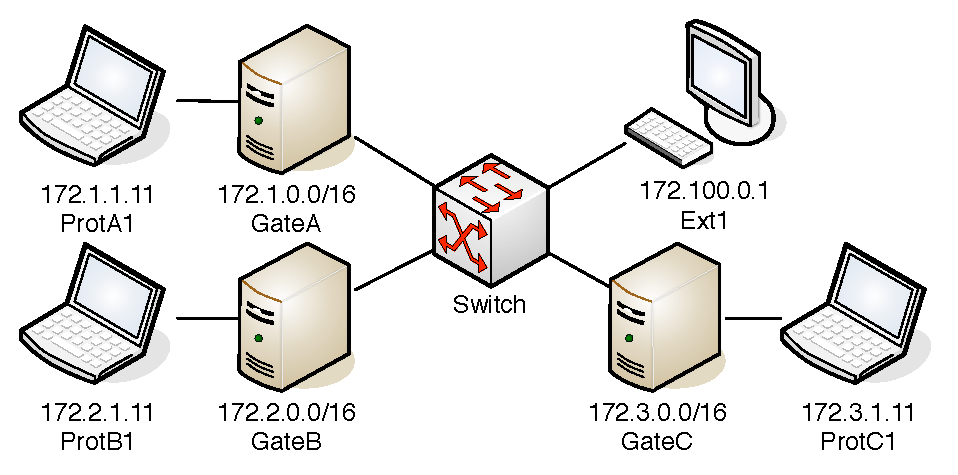
\includegraphics[width=0.75\textwidth]{../diagrams/thesis_network}
\end{figure}

\par Protected clients behind the gateways (\texttt{ProtA1}, \texttt{ProtB1}, and \texttt{ProtC1}) may communicate freely. The protected clients may also talk out to the external host (\texttt{Ext1}), and the external hosts must then---once that connection is established---be able to talk back into the network. There is additional administrative traffic directly between the gateways (\texttt{GateA}, \texttt{GateB}, and \texttt{GateC}). These three basic traffic flows are ``valid'' traffic.

\par All traffic beyond what is described above is ``invalid.'' For example, \texttt{Ext1} is not allowed to send traffic in to the protected clients or the gateways without them first initiating the connection. Malformed traffic sent by any host is also considered invalid. In either case, invalid traffic should be stopped at the earliest possible opportunity (i.e., the gateway rejects the packet and keeps it from reaching the internal host) and the system must remain stable.

\par To collect data, each system runs the traffic collection program \texttt{tcpdump} to capture the traffic sent and received into \ac{PCAP} files. Traffic generators are then spawned as appropriate on each system in the network, each of which logs their sends and receives. After a given trial, the \ac{PCAP} files and traffic generator logs are collated and processed with custom scripts to determine the metrics described in Section \ref{sec:metrics}. More details on the traffic generators and test run sequence can be found in Appendixes \tbd{ref the appendixes} and \tbd{other one}, respectively.

\par \tbd{implementation details on traffic generators and analyzers IN AN APPENDIX. Document EXACTLY how things happen in each test?}

\par All trials run on physical network on eight servers. Each server runs Ubuntu 12.04.1 Server Edition.

\section{Experimental Design}
\label{sec:exp_design}
\par Based on the factors given in Section \ref{sec:factors} and the goals of this research, as layed out in Section \ref{sec:goals}, there are nine traffic flows of interest. Each consists of different types of traffic and flow destinations. There are most easily visualized in Figure \ref{fig:testnum_flows}.

\tbd{create composite figure of each of the possible tests. Label each with the appropriate text number.}

\par These possible traffic flows are used in four sets of experiments, given below. Each experiment set answers a different research goal.
\begin{itemize}
	\item Basic tests
	\par This sequence of tests validates that \ac{ARG} classifies traffic correctly by running every traffic flow against \ac{ARG}. Latency is set to 20ms for all tests and traffic generators produce packets around every 0.3 seconds (actual traffic rate is higher due to responses and \ac{TCP} acknowledgement packets). To determine if hop rate has an expectedly large impact on certain types of traffic, a slow hop rate (500ms) and one close to double the latency (50ms).

	\item Max packet rate
	\par This sequence gives an indication of what packet rate \ac{ARG} is capable of handling. Packet rate goes through all levels shown in Table \ref{tbl:factors}. Hop rate changes between 500ms and 50ms to see if the additional \ac{IP} calculation load impacts the maximum rate. Test 4 \tbd{four?} is used in all runs to exercise all possible valid traffic flows. Latency is set to 20ms.

	\item Max hop rate
	\par This sequence determines the maximum hopping rate at various latencies. Hop rate and latency go through the levels shown in Table \ref{tbl:factors} in a full factorial fashion (every latency-hop rate combination). Packet rate is fixed at 0.3 seconds and Test 4 is used throughout.

	\item Fuzzer
	\par This sequence is not tested rigorously for traffic flow success and failure, but ensures that \ac{ARG} remains stable despite malformed traffic. Hop rate varies between 500ms and 50ms, latency is fixed at 20ms, and packets are sent at 0.3 second intervals.
\end{itemize}

\par Due to the possible impact of large network traffic disruptions, a 99\% confidence interval is used. Wide variation is possible in the actual traffic seen in a single run, so 10 replications are used for each experiment.

\section{Summary}
\label{sec:method_summary}
\tbd{don't need this section? Edit if we do}

\par This research determines if \ac{DYNAT}---the use of a gateway with a rapidly changing external \ac{IP} address---can effectively determine whether traffic should be allowed into a network. Several previous research efforts in this area already proved that \ac{DYNAT} made it more difficult to gain knowledge of a network \cite{BBNDYNAT} and that performance could be minimally impacted \cite{NAH}. 

\par A test network composed of two \ac{DYNAT}-protected networks and a few external hosts is used to explore this question. The custom \ac{DYNAT} solution used here, known as \ac{ARG}, allows the tuning of important system parameters. For the sake of this research, the primary factor is the hop rate. Levels used for experimentation include multiple times a second hops, several times a minute, and no hopping at all. Outside of \ac{ARG} itself, most hosts on the network run traffic generation scripts to simulate network activity. These scripts allow for the adjustment of packet rate, proportion of ``valid'' or ``invalid'' traffic produced, and how much traffic flows between the protected networks verses to the external hosts.

\par All hosts run the packet capture utilities, allowing custom analysis tools to run through each host's logs and pull out the desired metrics. For the research question posed above, the metrics include the overall rejection/acceptance rate of packets, incorrect classification of packets, and why packets are typically rejected. The factors and levels discussed in Section \ref{sec:factors} and the 10 replications result in 810 total experiments.

